\section{级数的收敛}
\label{sec:analysis-series}

有限和可以逐项相加，无限多项却无法“加完”。上一节的数列极限提供了处理办法：
把前$N$项的和看成一个数列，再问$N$无限增大时它是否趋向一个确定的数。
本节先用部分和定义级数及其收敛，再给出几何级数、裂项级数与$p$级数这些可作基准的例子；
随后分正项级数和变号级数建立收敛判别；最后说明改变求和次序与合并相邻项会怎样影响收敛和级数的和。

\subsection{级数的定义}
\label{sec:analysis-series-definition}

\paragraph{部分和}
给定数列$(a_n)_{n\geq1}$，把有限和的上限不断增大，就得到一个新的数列
\[
 s_N=\sum_{n=1}^{N}a_n=a_1+\cdots+a_N,
\]
$s_N$称为\term{部分和}（partial sum）。

\paragraph{无穷级数及其收敛}
符号\term{无穷级数}（infinite series）$\sum_{n=1}^{\infty}a_n$描述这一求和过程；
当$(s_N)$有有限极限$s$时，称级数收敛，并记$\sum_{n=1}^{\infty}a_n=s$；否则称级数发散。
例如$a_n=2^{-n}\to0$，而部分和$s_N=1-2^{-N}\to1$；
单项的极限与级数的和是两个不同的对象。

由$a_N=s_N-s_{N-1}$及差的极限法则可知，级数收敛必须有$a_N\to0$。反向则不成立：
上一节柯西数列部分的例子说明，调和级数$\sum_{n=1}^\infty1/n$的单项趋于零，部分和却不是柯西数列，因而发散。

级数是否收敛与前有限项无关：对任一固定的$m$，$\sum_{n=1}^\infty a_n$收敛当且仅当尾部$\sum_{n=m+1}^\infty a_n$收敛，
因为两者的部分和只相差固定的有限和$s_m$。此时$r_m=\sum_{n=m+1}^\infty a_n=s-s_m$称为余项，且$m\to\infty$时$r_m\to0$。

\paragraph{非负项级数的总和}
若所有$a_n\geq0$，部分和单调不减，因此有界时收敛，无界时趋于$+\infty$。
这种情形下统一记
\[
 \sum_{n=1}^{\infty}a_n:=\sup_N\sum_{n=1}^{N}a_n\in[0,+\infty].
\]
这是非负项级数的扩展总和；总和为$+\infty$时仍称级数发散，不把它混同于有限和。
这个记号对每个非负项级数都有意义，后面比较、重排和分组非负项时，都可以先在$[0,+\infty]$中比较总和，不必事先知道级数收敛。

\subsection{常见的级数}
\label{sec:analysis-common-series}

判断一般级数时，常把它与几类已经算清的级数比较。下面依次给出可以直接求和的几何级数与裂项级数，
以及收敛性由指数决定的$p$级数。

\paragraph{几何级数}
第~\ref{chap:sets-functions-and-proofs}章的有限几何和公式~\eqref{eq:prelim-finite-geometric-sum}给出$r\neq1$时
\[
 \sum_{n=0}^{N}r^n=\frac{1-r^{N+1}}{1-r}.
\]
当$|r|<1$时，前面的等比数列极限使$r^{N+1}\to0$，因而
\begin{equation}
 \sum_{n=0}^{\infty}r^n=\frac{1}{1-r}.
\label{eq:analysis-geometric-series}
\end{equation}
同一计算给出截断后的误差
$|\sum_{n=N+1}^{\infty}r^n|=|r|^{N+1}/|1-r|$。
若$|r|\geq1$，则$|r^n|\geq1$，单项不趋零，故级数发散。
几何级数既是一个可直接计算的例子，也提供比较其他级数尾部的基准。

\paragraph{裂项级数}
若每一项都能写成相邻两项之差$a_n=b_n-b_{n+1}$，第~\ref{chap:sets-functions-and-proofs}章的裂项求和公式~\eqref{eq:prelim-telescoping-sum}给出
$s_N=b_1-b_{N+1}$。因此级数收敛当且仅当$(b_n)$有有限极限$b$，此时$\sum_{n=1}^\infty a_n=b_1-b$。
例如$\frac1{n(n+1)}=\frac1n-\frac1{n+1}$，$b_n=1/n\to0$，故$\sum_{n=1}^\infty\frac1{n(n+1)}=1$。
裂项级数的部分和可以精确写出，因而与几何级数一样，可用作比较其他级数的基准。

\paragraph{$p$级数}
对于$\sum_{n=1}^{\infty}n^{-p}$，相邻项的比值趋于$1$，仅看单步下降不易区分不同的$p$。
可以将有限和按$n=2^k,\ldots,2^{k+1}-1$分成区块。
若$p>0$，每块有$2^k$项，块内每一项都介于$(2^{k+1})^{-p}$与$(2^k)^{-p}$之间，乘以项数得
\[
 2^{-p}2^{k(1-p)}
 \leq\sum_{n=2^k}^{2^{k+1}-1}n^{-p}
 \leq2^{k(1-p)}.
\]
任一部分和$s_N$都不超过前$K+1$个整块之和$s_{2^{K+1}-1}$，其中$2^{K+1}-1\geq N$，所以对整块的估计控制了全部部分和。
这里只比较有限区块，尚未调用无穷级数的分组规则。

$p>1$时，右侧随$k$构成公比$2^{1-p}<1$的几何级数，于是每个部分和都不超过$1/(1-2^{1-p})$；
由非负部分和的单调性，级数收敛。$0<p\leq1$时，$2^{k(1-p)}\geq1$，每块至少为$2^{-p}$，累计任意多块便无界。
$p\leq0$时原级数的单项已不趋零。因此$p$级数恰在$p>1$时收敛；
特别地，调和级数$\sum_{n=1}^{\infty}1/n$发散。

\subsection{级数的收敛判别}
\label{sec:analysis-series-tests}

判断级数收敛，就是判断部分和是否有有限极限。非负项的部分和单调，可以用上界控制；
出现正负项后，还须区分绝对值累计有限与依靠抵消才收敛的两种情形。

\subsubsection{正项级数}

\paragraph{比较判别法}
几何级数与$p$级数已提供两个基准。对一般正项级数，可以先比较单项，
再用非负部分和的单调性把大小关系传递到总和。
若充分大的$n$都有$0\leq a_n\leq b_n$，则
$\sum b_n$收敛蕴含$\sum a_n$收敛；$\sum a_n$发散蕴含$\sum b_n$发散。
这称为比较判别法，有限个前项不影响收敛。
例如$n\geq1$时$1/[n(n+1)]\leq1/n^2$，由$p=2$的情形也可知前者的级数收敛。

单项比值趋于正常数时，也可以直接比较。
若$a_n,b_n>0$且$a_n/b_n\to c\in(0,\infty)$，则最终
$(c/2)b_n\leq a_n\leq(3c/2)b_n$，两级数因而同收敛或同发散，称为极限比较判别法。

\paragraph{比值判别法}
另一种比较从相邻项的比例入手。设$a_n>0$且$a_{n+1}/a_n\to r$。
当$r<1$时，可选$r<q<1$，使充分靠后都有$a_{n+1}\leq qa_n$，
逐次代入得到$a_{N+j}\leq a_Nq^j$，用几何级数比较便知收敛。
当$r>1$时，充分靠后的项递增而不趋零，级数发散；比值趋于$+\infty$亦同。
这称为比值判别法。

$r=1$时无法据此判断：收敛的$\sum1/n^2$与发散的$\sum1/n$
都有相邻项比值趋于$1$，必须另用比较等方法。

\subsubsection{变号级数}

\paragraph{绝对收敛与条件收敛}
项的正负交替或不规则变化时，部分和失去单调性，正负抵消也会影响累计。
若实数级数$\sum a_n$的绝对值级数$\sum|a_n|$收敛，称原级数
\term{绝对收敛}（absolute convergence）；若原级数收敛但$\sum|a_n|$发散，则称为条件收敛（conditional convergence）。
绝对收敛意味着即使不依赖抵消，累计的绝对贡献仍有限。
条件收敛则要求同时证明原级数收敛和绝对值级数发散；只知道后者，不能排除原级数也发散。

\paragraph{绝对收敛的判定}
判断绝对收敛只需对非负项级数$\sum|a_n|$使用比较或比值判别；若它收敛，原级数便必收敛。
理由是对$m>n$有
\[
 |s_m-s_n|\leq\sum_{k=n+1}^{m}|a_k|\leq\sum_{k>n}|a_k|,
\]
右侧是收敛非负级数的余项，与$m$无关且随$n$增大趋于零，故$(s_n)$满足柯西准则。
因此绝对收敛蕴含收敛，判断时不必先单独证明原级数收敛。
例如$\sum(-1)^{n+1}/n^2$由$p=2$的情形得到绝对收敛。

若级数和为$s$，在上式中令$m\to\infty$（若极限大于右侧的固定数，充分靠后的$|s_m-s_n|$也会大于它），得到
\[
 |s-s_N|\leq\sum_{n>N}|a_n|\longrightarrow0,
\]
即绝对尾和是截断误差的上界。

\paragraph{条件收敛的判定}
绝对值级数发散后，还须判断原级数中的抵消是否足以使部分和稳定。
最基本的条件是：$b_n\geq0$单调不增且$b_n\to0$时，
交错级数$\sum_{n=1}^{\infty}(-1)^{n+1}b_n$收敛，这称为Leibniz判别法。

其偶数部分和单调不减，奇数部分和单调不增，且每个偶数部分和都不超过任何奇数部分和。
因此偶数部分和以$s_1$为上界，奇数部分和以$s_2$为下界，两列分别收敛；
相邻的奇偶部分和之差$s_{2n+1}-s_{2n}=b_{2n+1}\to0$，两个极限因而相同。
给定误差后，奇偶两类下标的尾部分别满足要求，取较晚的起点即知原部分和收敛。
级数和位于任意一对相邻的奇偶部分和之间，因此余项绝对值不超过$b_{N+1}$。

例如$\sum(-1)^{n+1}/n$收敛，绝对值级数却是调和级数，所以条件收敛。
若$\sum b_n$本来就收敛，Leibniz条件给出的交错级数则是绝对收敛，不能一概称为条件收敛。

更一般地，若$A_N=\sum_{n=1}^{N}a_n$一致有界，即存在$M$使$|A_N|\leq M$对所有$N$成立，
而$b_n\geq0$单调趋零，则$\sum a_nb_n$收敛，这称为Dirichlet判别法。
这里$a_n$提供有界振荡，$b_n$使振荡的权重趋零。

为说明二者如何配合，对$m\leq k$记$A_k^{(m)}=\sum_{n=m}^{k}a_n=A_k-A_{m-1}$，则$|A_k^{(m)}|\leq2M$。
把$a_k=A_k^{(m)}-A_{k-1}^{(m)}$代入有限和并整理，得到
\[
 \sum_{k=m}^{N}a_kb_k
 =A_N^{(m)}b_N+
   \sum_{k=m}^{N-1}A_k^{(m)}(b_k-b_{k+1}),
 \qquad A_{m-1}^{(m)}=0.
\]
由于$b_k-b_{k+1}\geq0$，这段和的绝对值不超过
$2M[b_N+\sum_{k=m}^{N-1}(b_k-b_{k+1})]=2Mb_m$，它与$N$无关且随$m$增大趋于零，由柯西准则得证。

取$a_n=(-1)^{n+1}$便回到交错情形。
该判别只保证原级数收敛；是否条件收敛，还须另外证明$\sum|a_nb_n|$发散。

图~\ref{fig:analysis-process-series-terms-sums}并排比较级数的项与部分和。两列项都趋零，累计后的行为仍然不同。
\begin{figure*}[!htbp]
 \centering
 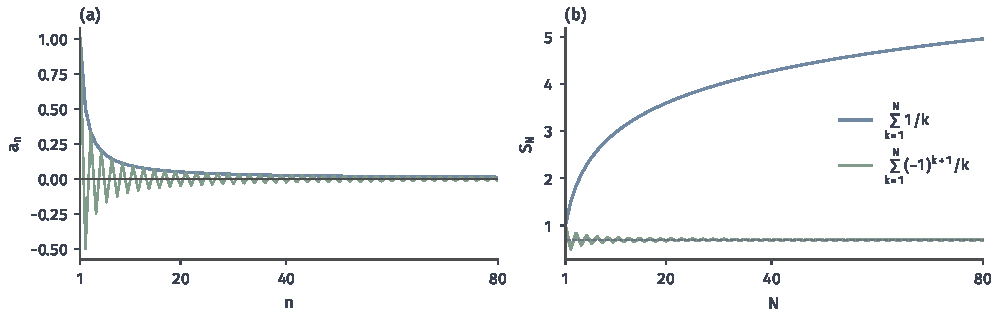
\includegraphics[width=169.0mm]{figures/00-shared/mathematical-preliminaries-upper/00-shared/matplotlib/chapter3-concept-processes/series-terms-sums.pdf}
 \caption{(a) 蓝、绿折线分别连接$1/n$与$(-1)^{n+1}/n$的前80项。(b) 对应的部分和：调和部分和继续增长，交错调和部分和趋于虚线所示的$\log2$。项趋零只是级数收敛的必要条件；图展示有限段，收敛或发散由前面的判别证明。}
 \label{fig:analysis-process-series-terms-sums}
\end{figure*}

\subsection{级数的重排和分组对收敛的影响}
\label{sec:analysis-series-rearrangement-grouping}

收敛判别处理的是原次序下的部分和。接下来改变求和的组织方式：重排改变各项的次序，
分组只把原次序中的有限个相邻项合并；两种操作对收敛性的影响不同，需要分别检验。

\paragraph{级数的重排}
有限和可以交换项的先后；无穷级数则要检查新的部分和如何覆盖旧项。
若$\pi:\{1,2,\ldots\}\to\{1,2,\ldots\}$为双射，$\sum_{n=1}^{\infty}a_{\pi(n)}$称为原级数的重排，
它每项恰好使用一次，改变的是各项进入累计的顺序。

对于非负项，重排的每个部分和只含有限个原下标，这些下标都不超过某个$N$，所以它不超过$s_N$，从而不超过原扩展总和；
反过来，原来的任意前$N$项也会全部进入重排的某个有限前段。对两个方向分别取上确界，便知重排保持总和，允许总和为$+\infty$。

绝对收敛也保证任意重排保持原和。设原级数和为$s$，记重排的部分和为$t_K=\sum_{n=1}^{K}a_{\pi(n)}$。
给定$\varepsilon>0$，先选$N$使$\sum_{n>N}|a_n|<\varepsilon$，再选$K_0$使$\pi(1),\ldots,\pi(K_0)$已包含$1,\ldots,N$。
当$K\geq K_0$时，$t_K-s_N$是若干个下标大于$N$的项之和，故$|t_K-s_N|\leq\sum_{n>N}|a_n|<\varepsilon$；
又由前面的截断误差界，$|s_N-s|<\varepsilon$。因此$|t_K-s|<2\varepsilon$，重排仍收敛到$s$。

条件收敛没有这一保证。记$P_N$、$Q_N$分别为前$N$项中正项之和与负项绝对值之和，
$P$、$Q$为相应的扩展总和。若其中一个有限，由$s_N=P_N-Q_N$收敛会推出另一个也有限，
于是$\sum|a_n|=P+Q$有限，与条件收敛矛盾，故二者都为$+\infty$。

对任意实数目标$L$，可以按原先的相对次序取正项，直到部分和超过$L$，
再取负项直到低于$L$，如此反复；每次都至少取一项相应符号的项。
由于$P=Q=+\infty$，每一轮都会在有限步内结束，两类项最终都被用到；
而$a_n\to0$使每次越过$L$的幅度趋零，因此得到和为$L$的重排。
原级数若含零项，每轮再按原次序插入下一个尚未使用的零项（若有）；这不改变和，并保证每个零项也最终被用到。
也可交替超过$1$、低于$0$，构造不收敛的重排。
可见条件收敛级数的和依赖抵消的顺序，不能按有限和的交换律任意调换。

\paragraph{级数的分组}
分组保持原项的顺序，只将有限个相邻项合为一项。
准确地说，取$0=n_0<n_1<n_2<\cdots$，令
$b_j=\sum_{k=n_{j-1}+1}^{n_j}a_k$，则分组后前$J$项的和恰为$s_{n_J}$。
所以原级数收敛到$s$时，分组后的部分和是原部分和的子序列，也必收敛到$s$；
这对绝对收敛和条件收敛都成立。

反向不成立。级数$1-1+1-1+\cdots$的部分和在$1$与$0$之间交替，原级数不收敛，
但按$(1-1)+(1-1)+\cdots$分组后各项为零。
分组只保留部分截断位置，可能掩盖块内的振荡。

非负项没有这种抵消：原部分和单调，分组截断又越过每一个原截断位置，
两者的上确界相同，故即使总和为$+\infty$也可保序分组。
结合非负项的重排规则，可先把非负项按任意编号排列，再分成有限相邻块，而不改变扩展总和；
后面构造外测度时，将用这些求和性质累计覆盖区间的长度。

\FloatBarrier
